\chapter{系统软件设计}

本章基于``Linux视觉端+云台主控+底盘主控''的分布式实现方案，围绕``感知-决策-执行''闭环，阐述系统软件架构、跨节点协同流程、控制算法、通信协议及异常处理机制。与单机式流程描述不同，本章侧重说明多控制器协同场景下的可复现实装路径，即各功能模块在Linux与MCU异构平台上的职责边界与相互之间的交互方式。

\section{软件总体架构与流程}

\subsection{程序分层与任务划分}

本课题的软件方案采用分布式分层架构，系统由三个相互独立但协同工作的计算节点构成：

（1）\textbf{Linux视觉节点}：承担目标检测与识别、目标状态管理及视觉数据封装输出等任务；

（2）\textbf{云台主控节点（STM32）}：负责IMU数据融合、双轴伺服控制、瞄准解算与云台执行闭环；

（3）\textbf{底盘主控节点（独立单片机）}：负责路径循迹、速度闭环、转向计数与圈次任务执行。

从功能维度出发，可进一步划分为以下五层：

（1）\textbf{设备驱动层}：实现RS485电机通信、IMU数据解码与串口数据接收，核心模块包括\texttt{drv\_ms4010}、\texttt{hipnuc\_dec}及\texttt{usart\_dataparsing}。

（2）\textbf{运动控制层}：由\texttt{laser\_gimbal}模块完成双轴角度控制、速度控制、坐标指向、回零与限位管理。

（3）\textbf{视觉追踪层}：Linux侧负责目标检测与状态跟踪，云台侧\texttt{laser\_gimbal\_vision\_tracker}模块完成像素误差闭环、目标状态机切换与自动搜索逻辑。

（4）\textbf{系统集成层}：在\texttt{main.c}、\texttt{laser\_gimbal\_test.c}与\texttt{laser\_gimbal\_vision\_test.c}中完成云台侧模块的初始化与运行控制，同时通过串口或总线协议与Linux视觉端及底盘主控端进行数据协同。

（5）\textbf{调试交互层}：通过MSH命令导出接口实现在线参数整定与功能验证，支撑不同场景下的快速迭代开发。

上述``节点解耦+功能分层''的设计将视觉计算负载、姿态控制任务与底盘实时控制任务分散至各自最适宜的平台，在降低单节点计算压力的同时提升了系统的可扩展性与工程可维护性。

\subsection{软件主流程图}

分布式系统主流程遵循“节点自检-链路建立-闭环协同”的启动顺序：

（1）\textbf{底盘节点启动}：完成电机、编码器、灰度传感器初始化，进入待命模式；

（2）\textbf{云台节点启动}：初始化GPIO与基础外设，调用\texttt{laser\_gimbal\_system\_init}完成电机管理器建立、电机扫描、云台参数绑定、电机使能与回零；

（３）\textbf{视觉节点启动}：Linux侧加载视觉模型与目标管理模块，基于嵌入式视觉系统框架与轻量化实现经验\cite{Liu2018DeepLearning}，建立与云台主控的数据通道并开始输出目标信息；

（4）\textbf{闭环协同运行}：云台节点持续接收视觉目标输入与IMU状态量，计算双轴控制量并执行瞄准；底盘节点独立执行循迹与速度闭环，同时按任务状态与上层指令完成机动。
系统总体程序流程图如图\ref{fig:program-flow}所示，左侧为视觉与云台控制链路，右侧为底盘循迹控制链路，两条链路并行运行、通过接口协同。

\begin{figure}[htbp]
\centering
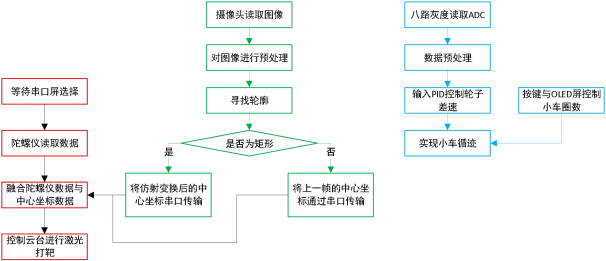
\includegraphics[width=0.95\textwidth]{images/chapters/fig-program-flow.png}
\caption{系统总体程序流程图}
\label{fig:program-flow}
\end{figure}
上述启动流程体现了``分布式职责清晰、局部闭环自治、跨节点协议协同''的工程原则：即使某一节点发生短时降级，其余节点仍可维持各自的最小功能闭环，从而提升了系统鲁棒性并降低了联调复杂度。

\section{IMU数据处理程序}

\subsection{数据采集与滤波}

系统通过\texttt{hipnuc\_dec}模块对HiPNUC协议进行字节流解码，先执行帧同步与CRC校验，再按数据包类型提取角速度、姿态角与加速度。数据解析成功后，角速度\(\omega\)与姿态角\(\theta\)被发布到控制路径供补偿计算使用。

在实现层面，工程采用“协议解码+阈值抑噪”策略：对小幅波动进行死区处理，避免将传感噪声直接放大到执行端。

\subsection{姿态解算与角速度发布}

系统在追踪线程中读取IMU实时状态，并构建前馈补偿项。以偏航轴为例，控制输出如式\eqref{eq:imu-feedforward}所示，该结构参考自抗扰控制思想\cite{Han2009ADRC}，在传统PID外环基础上叠加角速度与加速度前馈项：

\begin{equation}
u_{yaw}=u_{pid}+k_v\cdot \omega_{yaw}+k_a\cdot \dot{\omega}_{yaw}+k_x\cdot a_x
\label{eq:imu-feedforward}
\end{equation}

其中，\(u_{pid}\)为视觉误差闭环输出，\(\omega_{yaw}\)为角速度项，\(\dot{\omega}_{yaw}\)为角加速度近似项，\(a_x\)为加速度补偿项。该结构能够在平台突加速或抖动时提前修正执行量，降低纯视觉闭环的相位滞后影响\cite{Han2009ADRC}。

代码\ref{code:track-thread}展示了追踪控制线程的核心逻辑：每2\,ms一次（约500\,Hz）读取IMU数据计算前馈量，与视觉APID输出叠加后写入步进电机驱动器。

\begin{lstlisting}[style=cstyle, caption={视觉追踪线程与IMU前馈补偿（laser\_gimbal\_vision\_tracker.c）}, label=code:track-thread]
static void vision_tracker_thread_entry(void *parameter)
{
    vision_tracker_t *tracker = (vision_tracker_t *)parameter;
    float yaw_out = 0, pitch_out = 0;

    while (tracker->thread_running) {
        yaw_out = 0;  pitch_out = 0;

        if (tracker->enabled) {
            if (rt_mutex_take(tracker->tracker_mutex, 10) == RT_EOK) {
                /* 读取IMU角速度/加速度前馈量 */
                extern hipnuc_raw_t hipnuc_raw;
                float kv = kp_vel_yaw   * hipnuc_raw.hi91.gyr[2];
                float ka = kp_angle_yaw * hipnuc_raw.hi91.acc[0];

                /* 视觉APID外环输出 */
                vision_tracker_process_target(tracker,
                                              &yaw_out, &pitch_out);

                /* 叠加IMU前馈，补偿平台抖动 */
                yaw_out = yaw_out + kv + ka;

                vision_tracker_apply_control(tracker, yaw_out, pitch_out);
                rt_mutex_release(tracker->tracker_mutex);
            }
        }
        rt_thread_mdelay(2);   /* 控制周期 ~500 Hz */
    }
}
\end{lstlisting}

\section{视觉识别与跟踪程序}

\subsection{视觉线程架构与数据流}

视觉端采用"三线程+双队列"结构，该架构吸收了新一代实时跟踪与嵌入式跟踪思想\cite{zhang2024temporalcorrelationmeetsembedding}：

（1）\textbf{读取线程}\texttt{read\_thread\_func}：持续从摄像头读取帧，并通过\texttt{frame\_queue(maxsize=1)}仅保留最新一帧，降低处理时延累积；

（2）\textbf{处理线程}\texttt{process\_thread\_func}：完成颜色阈值分割、轮廓筛选、A4目标判别、PnP位姿解算与目标状态管理；

（3）\textbf{发送线程}\texttt{send\_thread\_func}：从\texttt{data\_queue}取出结果并按串口协议发送给云台主控。

该结构将“采集实时性”“算法计算量”和“通信阻塞风险”解耦，使视觉链路在高帧率下仍具备稳定吞吐。其核心数据路径可概括为：

\begin{equation*}
\text{Camera Frame}\rightarrow\text{HSV Segmentation}\rightarrow\text{Contour Filter}\rightarrow\text{PnP Pose}\rightarrow\text{Serial Packet}
\end{equation*}
读取线程核心代码如代码\ref{code:read-thread}所示，通过\texttt{maxsize=1}的有界队列确保处理端始终获取到最新帧，避免帧积压导致延迟累积。

\begin{lstlisting}[style=pythonstyle, caption={视觉读取线程（EDC\_Opencv.py）}, label=code:read-thread]
def read_thread_func(cap):
    """线程1：读取视频数据，仅保留最新一帧"""
    while running_event.is_set() and cap.isOpened():
        ret, frame = cap.read()
        if not ret:
            running_event.clear()
            break
        try:
            # 清空队列，确保只保留最新的一帧
            while not frame_queue.empty():
                frame_queue.get_nowait()
            frame_queue.put_nowait(frame)
        except queue.Full:
            pass  # 并发竞争时忽略
\end{lstlisting}

发送线程负责将处理结果格式化为\texttt{@x,y,flag,\#}协议帧并通过串口发送，核心代码如代码\ref{code:send-thread}所示。

\begin{lstlisting}[style=pythonstyle, caption={视觉发送线程与串口协议帧（EDC\_Opencv.py）}, label=code:send-thread]
def send_thread_func(ser):
    """线程3：从队列取结果并按协议发送"""
    while running_event.is_set():
        try:
            data = data_queue.get(timeout=1)
            # 固定帧格式：@x,y,flag,#
            msg = f"@{data['x']:.3f},{data['y']:.3f},{data['flag']:.1f},#"
            if ser and ser.is_open:
                ser.write(msg.encode('utf-8'))
        except queue.Empty:
            continue
\end{lstlisting}
\subsection{目标检测与几何筛选流程}

处理线程首先将图像统一到\(640\times480\)并进行高斯滤波，随后在HSV空间执行\texttt{inRange}二值化和开运算去噪。阈值由Trackbar在线调节并可写回\texttt{trackbar\_values.txt}，便于现场快速整定。

轮廓处理遵循“先粗筛、后精筛”策略：

（1）多轮廓合并：\texttt{merge\_close\_contours}按面积差与质心距离合并近邻轮廓，抑制边缘断裂造成的重复候选；

（2）几何约束：要求候选轮廓近似四边形，面积位于设定区间且宽高比满足约束；

（3）尺寸一致性校验：\texttt{find\_a4\_paper\_contours}利用\texttt{solvePnP}和重投影尺寸估计，判断候选是否与A4目标物理尺寸一致。

仅当上述条件同时满足时，目标才进入后续位姿解算与下发链路。该“形状+尺度”双重判据可显著降低误检。
几何筛选与PnP尺寸核查的关键代码如代码\ref{code:a4-filter}所示。函数先通过\texttt{solvePnP}解算位姿，再利用重投影尺寸估计与A4物理尺寸比对，拒绝误匹配的候选轮廓。

\begin{lstlisting}[style=pythonstyle, caption={A4目标PnP尺寸筛选（EDC\_Opencv.py）}, label=code:a4-filter]
def find_a4_paper_contours(contour, size_tolerance_mm=50):
    object_points = np.array([
        [-A4_WIDTH_MM/2, -A4_HEIGHT_MM/2, 0],
        [ A4_WIDTH_MM/2, -A4_HEIGHT_MM/2, 0],
        [ A4_WIDTH_MM/2,  A4_HEIGHT_MM/2, 0],
        [-A4_WIDTH_MM/2,  A4_HEIGHT_MM/2, 0]
    ], dtype="float32")
    ordered_pts = order_points(contour)
    (success, rvec, tvec) = cv2.solvePnP(object_points, ordered_pts,
                                          CAMERA_MATRIX, DIST_COEFFS)
    if success:
        distance_z_mm = tvec[2][0]
        if distance_z_mm < 100 or distance_z_mm > 2000:
            return False
        reprojected, _ = cv2.projectPoints(object_points, rvec, tvec,
                                            CAMERA_MATRIX, DIST_COEFFS)
        reprojected = reprojected.reshape(-1, 2)
        w_px = np.linalg.norm(reprojected[1] - reprojected[0])
        h_px = np.linalg.norm(reprojected[3] - reprojected[0])
        est_w = (w_px * distance_z_mm) / CAMERA_MATRIX[0, 0]
        est_h = (h_px * distance_z_mm) / CAMERA_MATRIX[1, 1]
        if (abs(est_w - A4_WIDTH_MM) < size_tolerance_mm and
                abs(est_h - A4_HEIGHT_MM) < size_tolerance_mm):
            return True
    return False
\end{lstlisting}
\subsection{PnP位姿解算与目标量生成}

在\texttt{perspective\_transform\_a4\_pnp}中，系统以A4纸四角的三维模型点与图像角点建立对应关系，调用\texttt{cv2.solvePnP}获得位姿向量\((rvec,tvec)\)。其中平移向量如式\eqref{eq:tvec}所示：

\begin{equation}
tvec=[T_x,T_y,T_z]^\top
\label{eq:tvec}
\end{equation}

据此可计算云台双轴角度指令，如式\eqref{eq:pan-tilt-angle}所示：

\begin{equation}
\theta_{pan}=\arctan\!\left(\frac{T_x}{T_z}\right),\qquad
\theta_{tilt}=\arctan\!\left(\frac{T_y}{T_z}\right)
\label{eq:pan-tilt-angle}
\end{equation}

并换算为角度输出。与此同时，程序还返回目标中心像素\((x,y)\)用于与云台侧像素闭环对接。

需要特别说明的是，当小车在运行过程中摄像头并非始终正对矩形目标时，目标在图像中会因透视关系产生严重的几何畸变，此时直接取检测到的四边形几何中心将引入系统误差。为此，本工程参考仿射变换校正策略：利用已知A4纸的宽高比，先对检测到的四边形执行透视变换，将其校正为标准比例的矩形后取中心点，再通过逆变换将中心坐标映射回原始图像坐标系，从而得到消除畸变影响的精确中心位置。该处理在PnP解算之前执行，可有效提升远距离或大视角偏转工况下的中心定位精度。

\subsection{丢失重捕获与串口通信协议}

工程通过\texttt{find\_target\_count}与\texttt{lose\_target\_count}实现轻量状态机：

（1）检测稳定阶段输出当前目标坐标；

（2）短时丢失阶段保持上次有效结果，避免控制突跳；

（3）持续丢失阶段回退到中心搜索点\((640,240)\)，并保留最近一次姿态估计作为过渡信息。

视觉端最终以固定格式发送：\texttt{@x,y,flag,\#}。其中\texttt{flag}用于表征当前帧目标状态，云台主控据此决定跟踪、保持或搜索策略。通过该协议，Linux视觉节点与STM32云台节点形成低耦合、可扩展的数据接口。

云台侧的串口帧解析通过状态机实现，代码\ref{code:uart-parser}展示了\texttt{Usart\_Dataparsiring\_Handle}中逐字节处理\texttt{@...{\#}}帧的核心逻辑。

\begin{lstlisting}[style=cstyle, caption={串口协议帧解析状态机（usart\_dataparsing.c）}, label=code:uart-parser]
void Usart_Dataparsiring_Handle(Data_Parsiring_Typedef *data,
                                uint8_t rx_data)
{
    if (data->statue == 0 && rx_data == data->frame_start) {
        memset(data->frame_string, '\0', 100);
        data->frame_lenght = 0;
        data->statue = 1;                       // 进入帧接收状态
    } else if (data->statue == 1
               && rx_data != data->frame_end) { // 数据段
        data->frame_string[data->frame_lenght] = rx_data;
        data->frame_lenght++;
    } else if (data->statue == 1
               && rx_data == data->frame_end) { // 帧结束
        Usart_Dataparsiring(data);              // 解析并分类各字段
        // 将解析结果送入追踪器：float[0]=x, [1]=y, [2]=confidence
        vision_tracker_input_target(
            &g_vision_tracker,
            camera_data.data_buff.float_data[0],
            camera_data.data_buff.float_data[1],
            camera_data.data_buff.float_data[2]);
        data->statue = 0;                       // 复位等待下一帧
    }
}
\end{lstlisting}

\section{双闭环控制程序设计}

\subsection{像素误差外环PID}

外环以图像中心偏差为输入，通过APID控制器计算期望角速度输出。其核心目标是：

（1）降低稳态指向误差；

（2）在目标横向快速移动时维持可接受的动态超调；

（3）与内层补偿项协同，避免高频振荡。

通过限制PID输出与偏差死区，工程在可达性与稳定性之间取得了折中。

\subsection{IMU角速度前馈内环}

内层以IMU角速度及其变化率作为前馈项直接叠加控制输出，对平台机动扰动进行快速抵消。与仅依赖视觉误差的策略相比，该方法对高动态工况更鲁棒，尤其在“目标仍在画面内但载体发生快速姿态变化”场景下，可显著减少跟踪偏差峰值。

此外，系统支持在线调节\texttt{vel\_kp}、\texttt{ang\_kp}、\texttt{acc\_kp}，便于在实车/实台架条件下快速完成增益整定。

代码\ref{code:vision-process}展示了追踪线程中像素误差到APID控制输出的核心计算流程：先将像素坐标偏差转换为角度误差，再经死区判断与APID计算生成双轴控制量。

\begin{lstlisting}[style=cstyle, caption={视觉追踪像素误差到APID控制输出（laser\_gimbal\_vision\_tracker.c）}, label=code:vision-process]
static rt_err_t vision_tracker_process_target(
        vision_tracker_t *tracker,
        float *out_yaw, float *out_pitch)
{
    float yaw_output = 0, pitch_output = 0;

    /* 像素坐标转角度误差 */
    float yaw_error_deg, pitch_error_deg;
    vision_tracker_pixel_to_angle_error(
        tracker,
        tracker->current_target.pixel_coord.x,
        tracker->current_target.pixel_coord.y,
        &yaw_error_deg, &pitch_error_deg);

    /* 死区判断：在死区内认为已锁定 */
    float pixel_dist =
        powf(tracker->current_target.pixel_coord.x
             - tracker->camera.center_x, 2) +
        powf(tracker->current_target.pixel_coord.y
             - tracker->camera.center_y, 2);
    if (pixel_dist < tracker->deadzone_pixels
                     * tracker->deadzone_pixels) {
        tracker->state = VISION_TRACK_STATE_LOCKED;
        vision_tracker_apply_control(tracker, 0, 0);
        goto FIX;
    }

    /* APID计算控制量 */
    uint32_t now = rt_tick_get_millisecond();
    yaw_output   = vision_pid_calculate(
                       &tracker->pid_yaw,   yaw_error_deg,   now);
    pitch_output = vision_pid_calculate(
                       &tracker->pid_pitch, pitch_error_deg, now);
FIX:
    *out_yaw   = yaw_output;
    *out_pitch = pitch_output;
    return RT_EOK;
}
\end{lstlisting}

\section{通信与上位机控制程序}

\subsection{USB-CDC通信协议}

工程通信分为两类：

（1）\textbf{执行链路通信}：MS4010电机通过RS485总线控制，底层完成命令打包、响应解析、校验和超时处理；

（2）\textbf{感知链路通信}：视觉前端通过串口发送目标像素数据，主控端解析后直接馈入追踪器。

其中，电机总线访问采用互斥锁串行化，避免多设备并发导致的帧冲突。

\subsection{Linux端控制界面与参数下发}

上位机可通过统一协议持续下发目标与参数，实现在线闭环调参与运行监控。尽管工程当前以嵌入式侧命令调试为主，但接口定义已具备扩展到Linux图形化参数面板的基础条件。

\section{系统主控程序设计与异常处理}

主控程序采用“初始化失败快速返回+运行期状态检查”的异常策略：

（1）初始化阶段：任一关键模块（电机管理器、电机发现、云台初始化、视觉追踪器初始化）失败即终止后续步骤并输出日志；

（2）运行阶段：通过状态机管理目标丢失、搜索、重捕获等过程，防止控制量无意义输出；

（3）并发保护：云台对象、追踪器对象与总线通信均设置互斥锁，降低资源竞争风险。

需要指出的是，部分代码中存在互斥保护被注释的情况，后续应统一临界区策略并补充高负载工况测试，以进一步提升系统稳定性。

\section{差速底盘工程的软件实现}

在本文分布式架构中，差速底盘控制被定义为与云台控制并行的独立子系统。为完善该子系统的软件实现，本文对参考目录下\texttt{WHEELTEC\_C07A\_IRF\_CAR}工程进行了代码级梳理。该工程围绕“红外感知-模式决策-差速执行”构建了可落地的循迹与定圈速运行闭环，可作为本系统底盘运动控制模块的直接实现依据。

\subsection{控制主循环与运行模式}

工程以定时中断作为核心控制时基，\texttt{Frequency=200}对应控制周期约\(5\,\mathrm{ms}\)。在中断中根据\texttt{Run\_Mode}执行不同控制分支：

（1）\textbf{停机模式}（\texttt{Run\_Mode=0}）：清零控制量并关闭驱动输出；

（2）\textbf{循迹模式}（\texttt{Run\_Mode=1}）：根据红外灰度结果生成\(Move\_X\)与\(Move\_Z\)；

（3）\textbf{转向模式}（\texttt{Run\_Mode=2}）：在路口阶段执行定向转弯，并在满足条件后回切循迹模式。

主循环（\texttt{empty.c}）负责传感器采样、归一化与状态触发，中断负责实时控制输出，这种“前台感知+中断闭环”的结构能够兼顾可读性和实时性。
代码\ref{code:chassis-irq}展示了定时中断内\texttt{Run\_Mode}分支的核心逻辑，包括一阶滞后滤波对偏差的平滑处理。

\begin{lstlisting}[style=cstyle, caption={底盘定时中断控制主循环（control.c）}, label=code:chassis-irq]
void TIMER_0_INST_IRQHandler(void)
{
    /* 5 ms 控制周期（Frequency = 200） */
    if (DL_TimerG_getPendingInterrupt(TIMER_0_INST)) {
        if (Run_Mode == 0) {          /* 停机模式 */
            Set_PWM(0, 0);
        }
        if (Run_Mode == 1) {          /* 循迹模式 */
            unsigned short Normal[8];
            if (Get_Normalize_For_User(&sensor, Normal)) {
                last_last_mid_value = last_mid_value;
                last_mid_value      = now_mid_value;
                now_mid_value       = gray_count_value(Normal);
                /* 一阶滞后滤波：抑制偏差突变引起的抖动 */
                now_mid_value = (int)(0.7f * now_mid_value
                              + 0.2f * last_mid_value
                              + 0.1f * last_last_mid_value);
                Move_X = fllow_speed;
                Move_Z = -(float)now_mid_value * turn_p;
            }
        }
        if (Run_Mode == 2) {          /* 转向模式 */
            Move_X = fllow_speed;
            Move_Z = turn_speed;
            if (++turn_count >= TURN_COUNT_MAX) {
                turn_count = 0;
                Run_Mode   = 1;       /* 回切循迹模式 */
            }
        }
        Get_Target_Encoder(Move_X, Move_Z);
        DL_TimerG_clearInterruptStatus(TIMER_0_INST,
                   DL_TIMER_INTERRUPT_ZERO_EVENT);
    }
}
\end{lstlisting}
\subsection{红外循迹与路口判别策略}

该工程使用8路灰度传感器，先通过\texttt{Get\_Normalize\_For\_User}得到归一化数据\texttt{Normal[8]}。随后通过两级判别实现路径跟踪：

（1）\textbf{偏差估计}：\texttt{gray\_count\_value()}采用加权法计算横向偏差，权重从左到右对称分布（负到正），可连续表征赛道中心偏移量；

（2）\textbf{路口检测}：\texttt{gray\_is\_turn()}按平均反射强度和前部传感器触发计数判断是否到达拐点/十字区域，并据此触发模式切换。

在循迹模式下，工程调用\texttt{IRDM\_line\_inspection()}将多种红外组合状态映射为转向指令，覆盖直行、小偏转、中偏转、大偏转及直角转等场景，从而提升复杂线路下的连续通过能力。

在灰度数据的处理流程上，工程对8路原始ADC输出进行了四级处理以提升控制丝滑度：均值滤波，对每路做多次采样平均，降低电气噪声；归一化计算，以黑白基准值为端点，将各路输出映射到$[0,1]$区间，消除传感器个体差异和安装高度变化的影响；加权偏差估计，对8路归一化值按位置权重相加求得横向偏差量，近中心传感器权重小、远端权重大，提高边缘感知灵敏度；一阶滞后滤波，对最终偏差量施加低通滤波$y_k = (1-\alpha)\,y_{k-1}+\alpha\,u_k$，防止偏差突变引起的云台/底盘抖动，保证整车运行平稳。

\subsection{固定圈速实现与圈数管理}

“固定圈速”在该工程中由“恒定前向速度+转弯计数”协同实现：

（1）\textbf{速度基准}：\texttt{fllow\_speed}作为循迹阶段前向速度基准，可通过按键在线增减；

（2）\textbf{转弯计数}：每次完成一次有效拐角后\texttt{turn\_number++}；

（3）\textbf{圈数终止}：当\texttt{turn\_number == round\_number*4}时判定完成设定圈数（默认按每圈4个关键转角计）。

该实现方式不依赖全局定位系统，工程代价低，适合教学与竞赛场景下的闭环里程/圈次任务。

\subsection{差速运动学与轮速闭环}

在执行层，系统先依据差速模型进行左右轮目标速度分解，再结合编码器反馈完成速度闭环控制。左右轮目标转速分解关系如式\eqref{eq:diff-kinematics}所示：

\begin{equation}
v_L = v_x - \frac{L}{2}\,\omega,\qquad
v_R = v_x + \frac{L}{2}\,\omega
\label{eq:diff-kinematics}
\end{equation}

其中，\(v_x\)为前向速度指令，\(\omega\)为角速度指令，\(L\)为轮距。工程中\texttt{Get\_Target\_Encoder()}负责该分解，\texttt{Incremental\_PI\_Left/Right()}完成增量式PI调节，\texttt{Set\_PWM()}输出电机PWM。轮速反馈由AB相编码器中断计数获得，实现“目标-测量-校正”的实时闭环。
代码\ref{code:chassis-pi}列出了差速分解函数与左轮增量式PI调速器的具体实现，PI输出量经双端饱和限幅后写入PWM寄存器，防止积分饱和导致控制量溢出。

\begin{lstlisting}[style=cstyle, caption={差速运动学分解与增量式PI调速（control.c）}, label=code:chassis-pi]
/* 差速运动学：将纵向速度/角速度分解为左右轮目标转速 */
void Get_Target_Encoder(float Vx, float Vz)
{
    if (Vx < 0) Vz = -Vz;  /* 倒退时角速度方向取反 */
    MotorA.Target_Encoder = Vx - Vz * Wheelspacing / 2.0f;
    MotorB.Target_Encoder = Vx + Vz * Wheelspacing / 2.0f;
}

/* 增量式PI调速：累积误差增量，双端限幅防积分饱和 */
int Incremental_PI_Left(float Encoder, float Target)
{
    static float Bias, Pwm, Last_bias;
    Bias = Target - Encoder;

    float bias_i = Velocity_KI * Bias;
    if (bias_i >  1000) bias_i =  1000;  /* 积分分量限幅 */
    if (bias_i < -1000) bias_i = -1000;

    Pwm += Velocity_KP * (Bias - Last_bias) + bias_i;
    if (Pwm >  6000) Pwm =  6000;       /* 输出总量限幅 */
    if (Pwm < -6000) Pwm = -6000;

    Last_bias = Bias;
    return (int)Pwm;
}
\end{lstlisting}
\subsection{作为系统子模块的协同与可靠性优势}

在本课题中，底盘子系统与云台子系统通过接口协同，而非控制耦合。WHEELTEC工程的实现经验表明，将底盘控制链路独立设计可带来以下优势：

（1）\textbf{互不干扰}：底盘循迹与云台瞄准分别在各自控制器内闭环运行，避免因单侧任务波动造成另一侧控制性能下降；

（2）\textbf{独立运行}：底盘可在无云台参与或云台暂时降级时继续完成机动任务，云台也可在底盘速度变化时维持自身姿态控制闭环；

（3）\textbf{可靠性更高}：故障被限制在子系统内部，便于隔离、诊断与恢复，系统整体可用性优于单控制器集中式方案。

工程实现层面，“模式状态机+事件触发”与“运动学分解+编码器PI”共同构成底盘侧基础控制框架。后续联调中，本文以标准化接口将其接入视觉与云台链路，形成“底盘机动-目标感知-指向执行”的分布式协同闭环。
\section{本章小结}

本章给出系统的软件总体架构与运行流程，明确了Linux视觉端、STM32云台主控与底盘主控的职责边界及协同流程，详细介绍了视觉线程设计、像素误差外环APID、IMU角速度前馈内环、通信协议与异常处理策略。文中还说明了初始化顺序、互斥保护与容错机制，以保证多节点并行时的实时性与可靠性。该软件框架为后续参数整定、联调验证与性能评估提供了系统化、可追溯的软件依据。
